\section{State redistribution in one dimension} \label{sec:srd1d}
We begin this section  by reminding the reader that cell merging can
be written as a postprocessing step. We then show that the extension of
cell merging for overlapping cells does not maintain conservation. This
provides the motivation for state redistribution, which is illustrated on
a simple example in one dimension to gain intuition without too much
notation.  Although the small cells do not mimic the cut cells at the 
boundary in higher dimensions, this is still a useful model problem. 

For the examples in this section we will solve the linear advection equation
\begin{equation}\label{eq:hpde}
u_t + au_x = 0, \quad a>0
\end{equation}
on the nonuniform grid, called the base grid. Equation \eqref{eq:hpde} is
discretized  using the  first order
accurate upwind scheme 
\begin{equation}\label{eq:unstable1d}
\widehat{U}_i = U^n_i - \frac{a \Delta t} {h_i} \, (U^n_i -U^n_{i-1}),
\end{equation}
where $U^n_i$ is the solution average on cell $i$ at time step $t^n$, the time
step $\Delta t$ is constant for all cells. On full cells, $h_i = h$ and on
the small cells,  and $h_i = \alpha h$ for $ 0 < \alpha < 1$.
We first use
the grid in Figure \ref{fig:ng1}(a) with one small cell at $i=0$, then the grid
in Figure \ref{fig:ng1}(b) with two small cells at $i = -1$ and $1$.

\begin{figure}[h]
\centering
\vspace*{.2in}
\mbox{
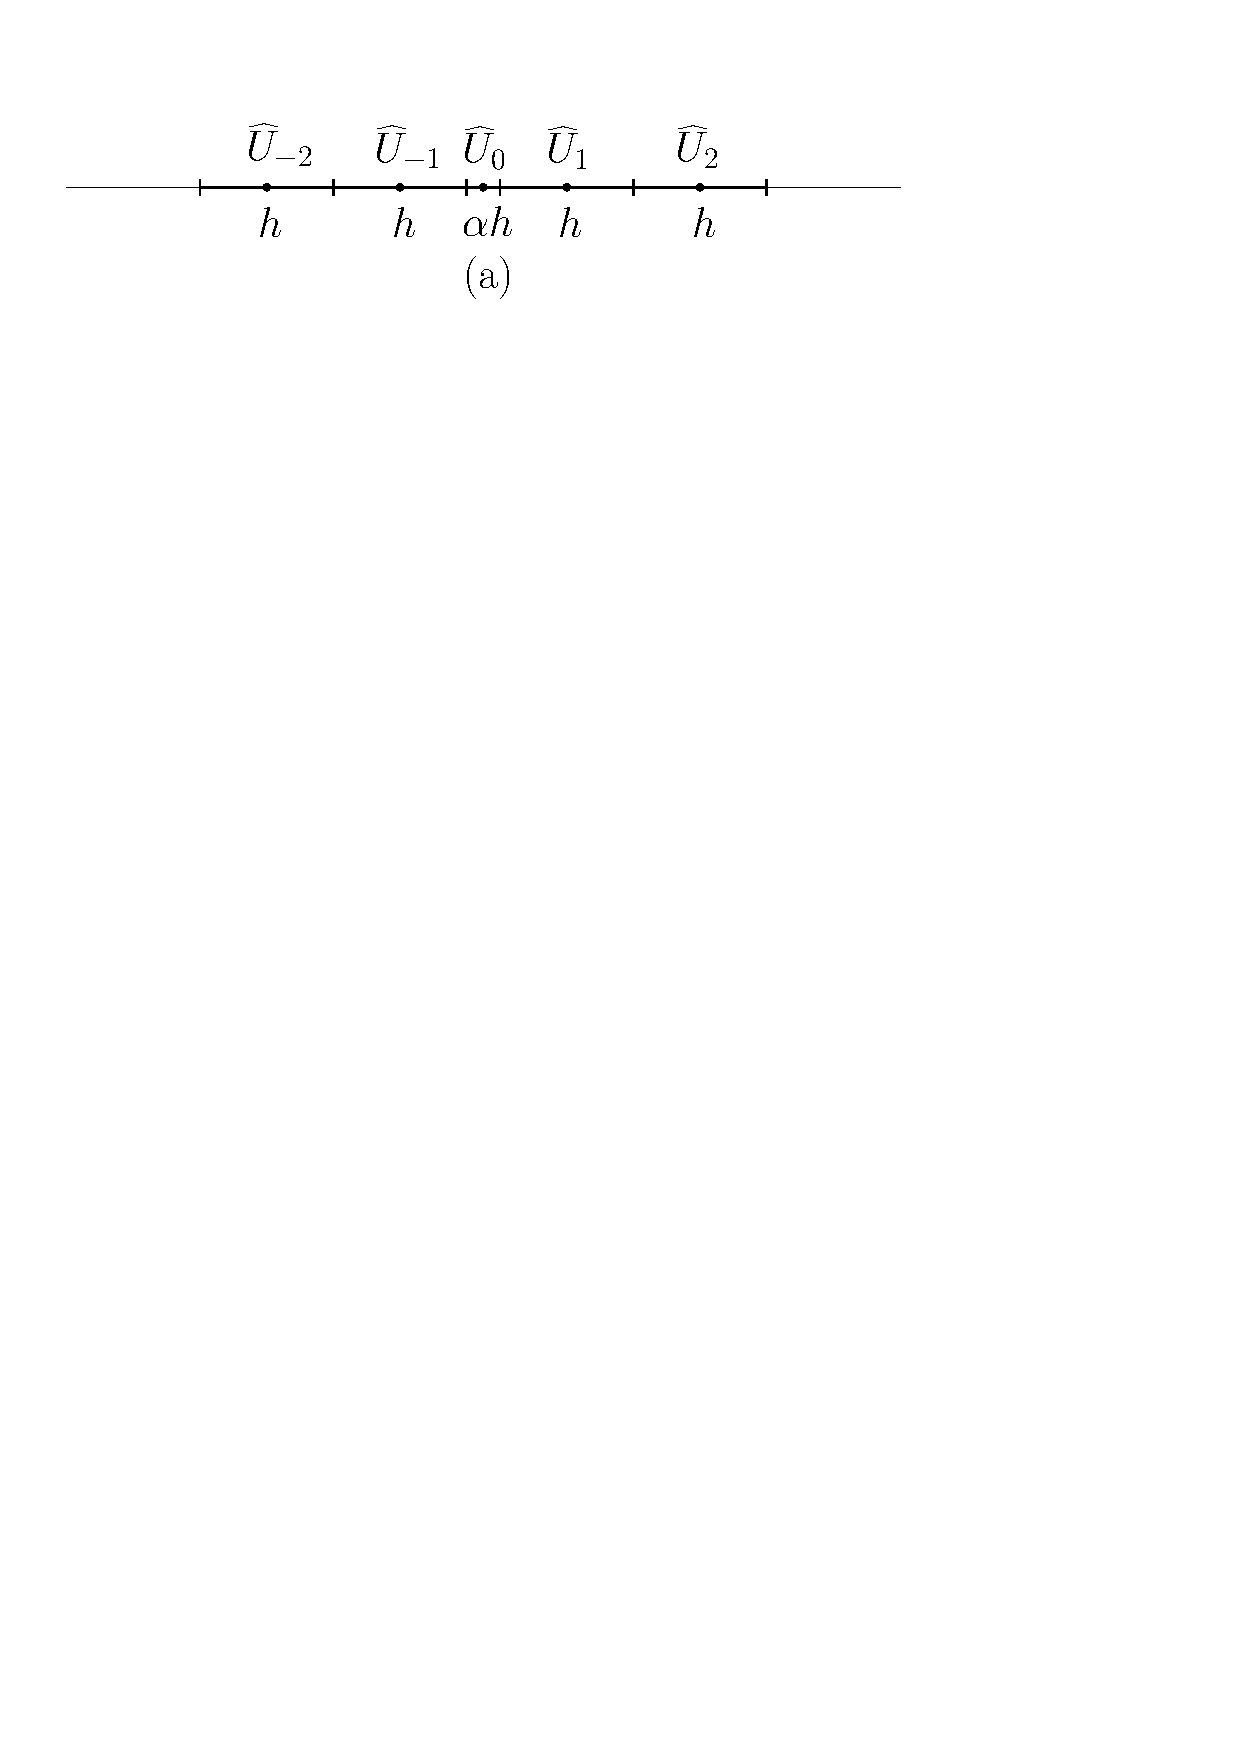
\includegraphics[width=0.4\linewidth,trim=30 0 20 0,clip]{figs/overlapping_simple.pdf} 
\hspace*{.1in}
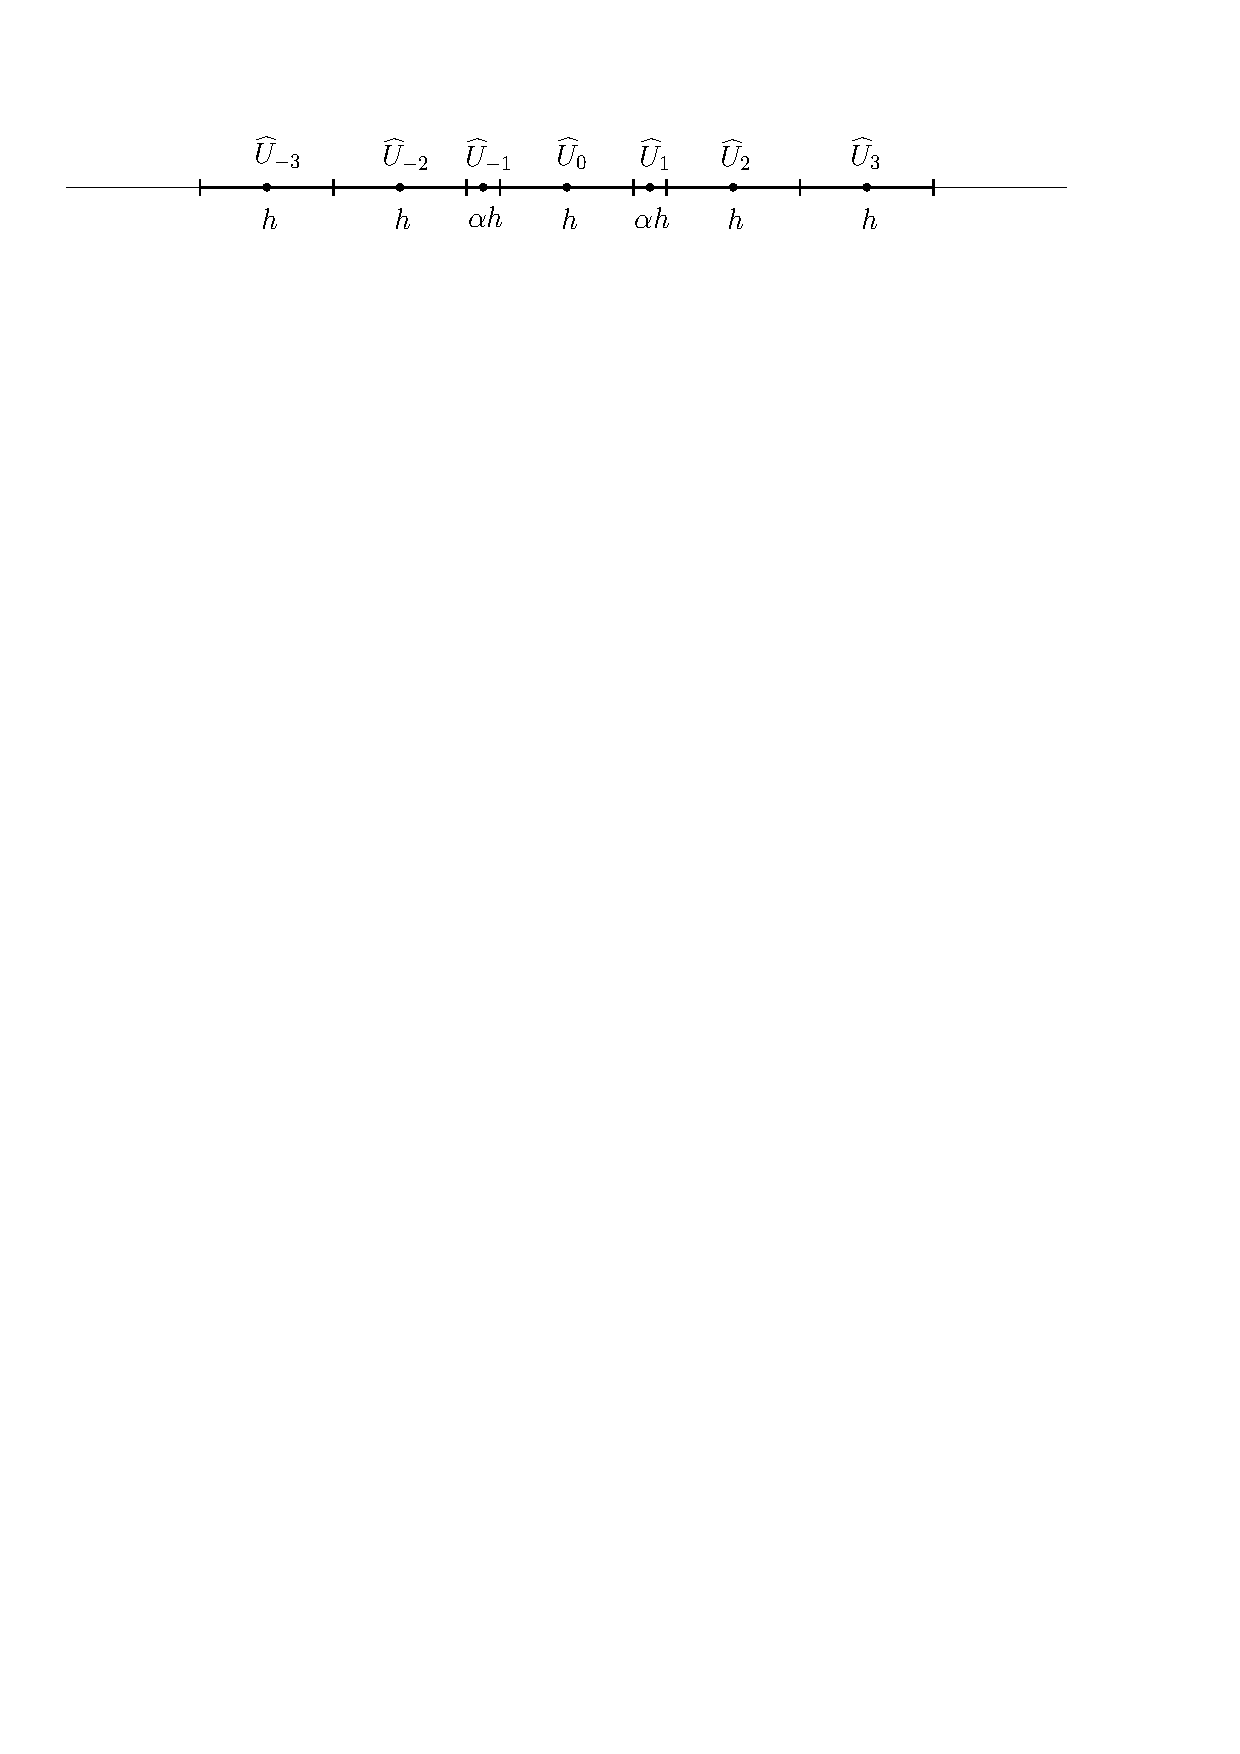
\includegraphics[width=0.5\linewidth,trim=15 0 25 0,clip]{figs/overlapping.pdf}
}
\vspace*{.1in}
\caption{\sf Model problem in one space dimension on nonuniform base grid.
On the left there is one small cell at $i=0$. The right grid has two small 
cells  at $i = -1$ and $1$.  The small and large cell 
sizes are $\alpha h$ ($0<\alpha < 1$), and $h$, respectively. \label{fig:ng1}}
\end{figure}

On the grid in Figure \ref{fig:ng1}(a), cell merging might look like this.
First, after the unstable update in \eqref{eq:unstable1d}, form the 
volume-weighted merged cell $\widehat{Q}_0$:
\begin{equation}
\widehat{Q}_0 = \frac{\widehat{U}_{-1} + \alpha \,  \widehat{U}_0 + 
\widehat{U}_1}{2+\alpha} .
\end{equation}
The cells comprising the merged cell
are then replaced by $\widehat{Q}_0$:
\begin{equation}
\widehat{U}_{-1}^{n+1} = \widehat{U}_0^{n+1} = \widehat{U}_1^{n+1} =
\widehat{Q}_0
\end{equation}
This is easily seen to be conservative by checking that
\begin{equation}
h \, (U_{-1}^{n+1} + \alpha \, U_0^{n+1} + U_1^{n+1})
= (2+\alpha) h \,  \, \widehat{Q}_0 =
 \, (\widehat{U}_{-1} + \alpha \, \widehat{U}_{0} +  \widehat{U}_{1})
\end{equation}
which equals the values at time $t^n$  except for the mass entering and
leaving this region.


Next, consider the more complicated case of Figure \ref{fig:ng1}(b).
Five cells (indexed by $-3$, $-2$, $0$, $2$, $3$) are large 
with size $h$ and the remaining two cells (indexed by $-1$ and $1$) 
are small with size $\alpha h$.
A first approach to cell merging on this grid
might be to make two merging neighborhoods, $\widehat{Q}_{-1}$
comprising $u_{-2},u_{-1},u_0$, and $\widehat{Q}_1$ comprising $u_0, u_1$ 
and $u_2$.
The first order version here would assign cells as before, except that
since cell 0 belongs to two neighborhoods, it seems  reasonable
to assign $u_0 = \frac{1}{2} (\widehat{Q}_{-1} + \widehat{Q}_1).$  
It can quickly be  seen however
that this is not conservative. 

This motivates the state redistribution
procedure, which allows for overlapping cells and stabilizes 
$\widehat{U}_i$ in a conservative manner.
This is done by temporarily merging cells of the grid into 
larger, possibly overlapping, neighborhoods using a specially weighted 
convex combination, and recombining these averages back onto the
grid in a particular fashion.  These merged cells are 
constructed once during a mesh preprocessing step before timestepping.

\begin{figure}[h]
\begin{center}
\vspace*{.1in}
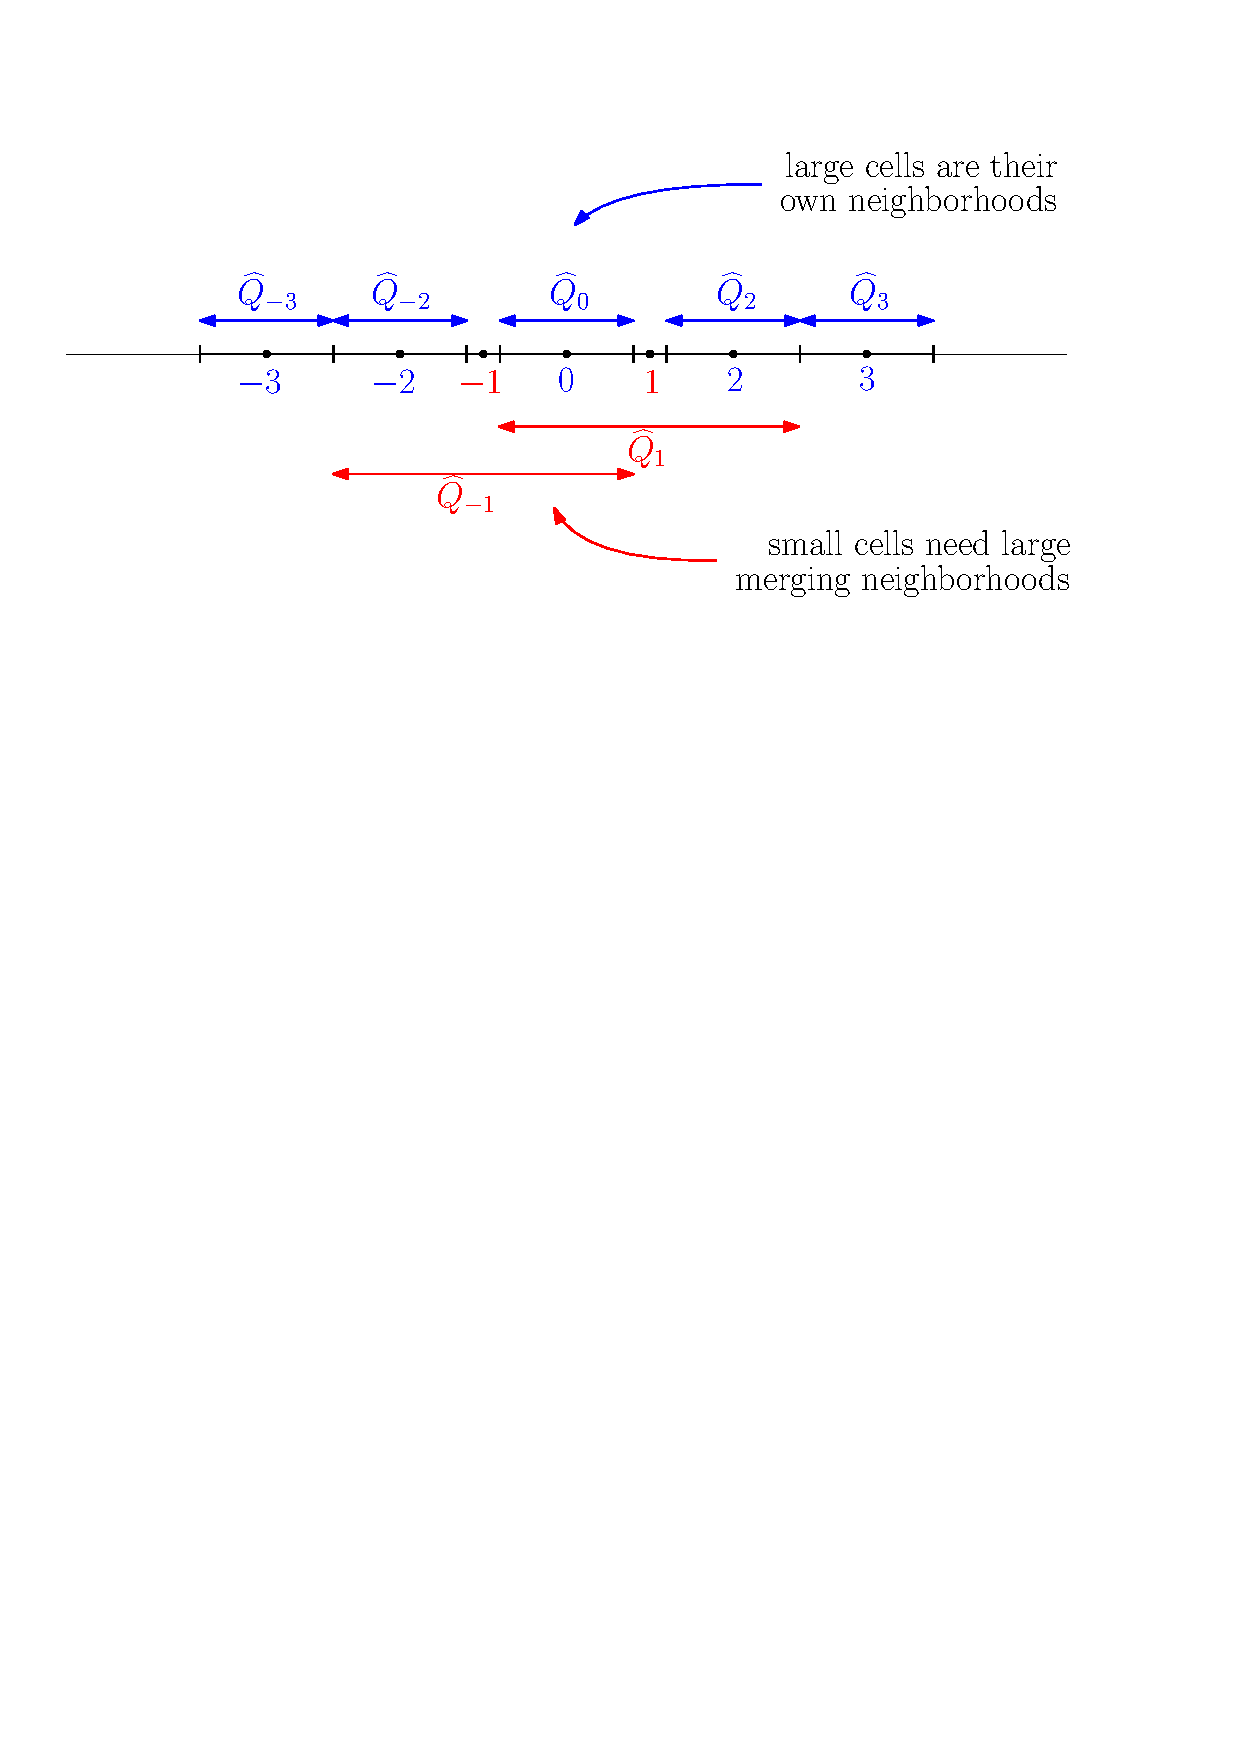
\includegraphics[width=0.75\linewidth]{figs/overlapping1.pdf} 
\caption{\sf 
The blue arrows indicate the merging neighborhoods associated to the large 
cells $-3$, $-2$, $0$, $2$, and $3$, which are their own neighborhoods.  
The red arrows indicate the neighborhoods of small cells $-1$ and $1$, which
have temporarily merged with their left and right neighbors.  
%The numbers next to the arrows are the neighborhood index, which
%correspond to the cell indices in Fig. \ref{fig:ng1}.  
\label{fig:mn1}}
\end{center}
\end{figure}

\subsubsection*{State redistribution preprocessing}
Each cell in the base grid (both large and small) has a merging neighborhood associated to it.
This is  a set of neighbors with which to temporarily merge.
Neighborhoods share the same index as the cell that generated it.
%The merging neighborhood associated to cell $i$ is called $M_i$. 
Small cells merge with their neighbors until the volume of the merging neighborhood is greater than
a threshold, taken here to be half the large cell size of $h/2$.
This is illustrated by the red arrows in Figure \ref{fig:mn1} where the merging neighborhood of 
small cell $-1$ consists of cells $-2$, $-1$, and $0$, and the merging neighborhood of 
small cell 1 consists of cells $0$, $1$, and $2$. 
A large cell does not need to merge with neighbors (since $h > h/2$), thus its merging neighborhood is only 
composed of itself.  This is illustrated by the blue arrows in Figure
\ref{fig:mn1}. For example,  the 
merging neighborhood of large cell $-3$ is composed only of itself.

Finally, each cell in the base grid counts the number of neighborhoods that overlap it. 
Cell $-2$ is overlapped by two neighborhoods, indexed by $-1$ and $-2$.
Cell 0 has 3 such neighborhoods, its own, and one from each small cell adjacent to it.

\subsubsection*{State redistribution postprocessing}
Using the above information we can now stabilize \eqref{eq:unstable1d} using the state redistribution 
method on the grid in Figure \ref{fig:ng1}.  
On each merging neighborhood, we compute a weighted solution average $\widehat Q_i$, where $i$ is the 
index of the merging neighborhood. 
$\widehat Q_i$ is computed by a convex combination of the averages $\widehat{U}_i$ of cells contained in the 
merging neighborhood, weighted by the inverse of the number of its overlap count. 
For example, on merging neighborhood $-1$, the weighted solution average is
\begin{equation}\label{eq:neigh2}
\widehat{Q}_{-1} = \frac{1}{\underbrace{h/2 + \alpha h + h/3}_{\text{weighted volume}}}\biggr( \underbrace{\frac{h}{2} \widehat{U}_{-2} + \alpha h \widehat{U}_{-1} + \frac{h}{3}\widehat{U}_{0}}_{\text{weighted mass}} \biggr).
\end{equation}
In formula \eqref{eq:neigh2}  for the weighted mass,
the cell volume is divided by the number of neighborhoods that overlap the associated cell 
in the base grid. 
For example, the multiplier in front of $\widehat{U}_{-2}$ is $\frac{h}{2}$ since there are 
two neighborhoods (from cells $-1$ and $-2$) that overlap cell $-2$.  
Similarly, the multiplier in front of $\widehat{U}_{-1}$ is $\alpha h$ since there is only 
one neighborhood (its own) that overlaps cell $-1$.
Finally, the multiplier in front of $\widehat{U}_{0}$ is $\frac{h}{3}$ since there are three neighborhoods that overlap cell $0$, i.e., cell $0$ is overlapped by neighborhoods $-1$, $1$, and $0$.
These multipliers are then divided by the weighted volume,  $(h/2 + \alpha h + h/3)$.
i%since $\widehat{Q}_{-1} $ must be a convex combination of $\widehat{U}_{-2}$, $\widehat{U}_{-1}$, and $\widehat{U}_{0}$.
The weighted solution average on merging neighborhood $1$ is similarly defined as
\begin{equation}\label{eq:neigh3}
\widehat{Q}_{1} = \frac{1}{h/2 + \alpha h + h/3}\left( \frac{h}{2} \widehat{U}_{2} + \alpha h \widehat{U}_{1} + \frac{h}{3}\widehat{U}_{0} \right).
\end{equation}
The weighted solution averages on merging neighborhoods that contain only one cell are simply 
\begin{equation}\label{eq:neigh1}
\widehat{Q}_i = \widehat{U}_i \quad \text{ for } i = -3,-2,0,2,3.
\end{equation}

The stabilized solution average at time $t^{n+1}$ on a cell in the base grid is then 
given by the average of all the weighted neighborhood averages that overlap it.  
On the cell overlapped by three neighborhoods we have
\begin{equation} \label{eq:threeneigh}
U^{n+1}_{0} = \frac{1}{3}(\widehat{Q}_{-1}+\widehat{Q}_{0}+\widehat{Q}_{1}).
\end{equation}
On the  cells overlapped by two neighborhoods, we have
\begin{equation} \label{eq:twoneigh}
U^{n+1}_{-2} = \frac{1}{2}(\widehat{Q}_{-1}+\widehat{Q}_{-2}) \text{ and } U^{n+1}_{2} = \frac{1}{2}(\widehat{Q}_{1}+\widehat{Q}_{2}).
\end{equation}
Finally, on cells overlapped by only one neighborhood,  we have
\begin{equation} \label{eq:oneneigh}
	U^{n+1}_i = \widehat{Q}_i \text{ for } i = -3,-1,1,3.
\end{equation}

We can write the final solution update on the small cells after SRD  at $t^{n+1}$ in terms of the solution 
averages at $t^{n}$, giving
\begin{equation}
\begin{aligned}
U^{n+1}_{-1} &= \frac{2-2\lambda}{5+6\alpha}U^n_0 + \frac{6\alpha - 4 \lambda}{5+6\alpha}U^n_{i-1}+ \frac{3\lambda + 3}{5+6\alpha}U^n_{i-2}+\frac{3\lambda }{5+6\alpha}U^n_{i-3}, \\
U^{n+1}_{1} &= \frac{2+4\lambda}{5+6\alpha}U^n_0 + \frac{6\alpha - 3 \lambda}{5+6\alpha}U^n_{i+1}+ \frac{3-3\lambda}{5+6\alpha}U^n_{i+2}+\frac{2\lambda }{5+6\alpha}U^n_{i-1}.
\end{aligned} \label{eq:finalupdate}
\end{equation}
Before application of the state redistribution method, the weights that multiply the solution averages at time $t^n$ in the base scheme \eqref{eq:unstable1d} become unbounded as $\alpha \rightarrow 0$.
However, after state redistribution this is no longer the case for the weights 
in \eqref{eq:finalupdate}.  This hints at the stability of our modified scheme.  

The state redistribution algorithm allows us to take full time steps as if there were no 
small cells in the grid.  However, it can be seen that the multipliers of $U^n_{i-1}$ and $U^n_{i+1}$ 
in \eqref{eq:finalupdate} are negative when $\alpha$ is small enough.  This means that our scheme is not 
monotone and thus not total variation diminishing.  We note that this is also the case for 
with flux redistribution, which has been successfully used in higher dimensions and more
compicated problems, 
so we are not concerned.
%about the application of SRD in
%higher dimensions and more complicated problems. 
The computational examples in Section \ref{sec:compResults} bear this out.  

\subsubsection*{Conservation}
We now show that our modified scheme \eqref{eq:threeneigh}, \eqref{eq:twoneigh}, \eqref{eq:oneneigh} conserves mass.
%, i.e., the total mass of the numerical solution before and after state redistribution is the same.  
For the portion of the grid in question, the total mass after state redistribution is
\begin{equation}\label{eq:tm1}
	\sum_{i} h_i U^{n+1}_i  = h U^{n+1}_{-3} + h U^{n+1}_{-2} + \alpha h U^{n+1}_{-1} +h U^{n+1}_0+\alpha h U^{n+1}_{1} + h U^{n+1}_{2} + h U^{n+1}_{3},
\end{equation}
where $h_i$ is the local cell size.
%i.e., $h_i = \alpha h$ for $i \neq -1,1$ and $h_i = h$ otherwise.
Substituting expressions for the final update \eqref{eq:threeneigh}, \eqref{eq:twoneigh}, \eqref{eq:oneneigh} into \eqref{eq:tm1}, we obtain
\begin{equation}\label{eq:tm2}
\begin{aligned}
\sum_{i} h_i U^{n+1}_i  &= h \widehat{Q}_{-3} + \frac{h}{2}(\widehat{Q}_{-1}+\widehat{Q}_{-2}) \\
&+ \alpha h \widehat{Q}_{-1} +h \frac{1}{3}(\widehat{Q}_{-1}+\widehat{Q}_{0}+\widehat{Q}_{1})+\alpha h \widehat{Q}_{1} \\
&+ h \frac{1}{2}(\widehat{Q}_{1}+\widehat{Q}_{2}) + h \widehat{Q}_{3}.
\end{aligned}
\end{equation}
Grouping terms in \eqref{eq:tm2}, we have
\begin{equation}\label{eq:tm3}
\begin{aligned}
\sum_{i} h_i U^{n+1}_i  &= h \widehat{Q}_{-3} + \frac{h}{2}\widehat{Q}_{-2} \\
&+ \left(\frac{h}{2}+\alpha h + \frac{h}{3}\right) \widehat{Q}_{-1} + \frac{h}{3} \widehat{Q}_0 + \left(\frac{h}{2}+\alpha h + \frac{h}{3}\right) \widehat{Q}_{1} \\
&+ \frac{h}{2}\widehat{Q}_{2} + h \widehat{Q}_3.
\end{aligned}
\end{equation}
Substituting the expressions for the neighborhood averages \eqref{eq:neigh3}, \eqref{eq:neigh2}, \eqref{eq:neigh1} into \eqref{eq:tm3}, we obtain
\begin{equation}\label{eq:tm4}
\begin{aligned}
\sum_{i} h_i U^{n+1}_i  &= h \widehat{U}_{-3} + \frac{h}{2}\widehat{U}_{-2} \\
&+ \left(\frac{h}{2} \widehat{U}_{-2} + \alpha h \widehat{U}_{-1} + \frac{h}{3}\widehat{U}_{0}\right) + \frac{h}{3} \widehat{U}_0 + \left(\frac{h}{2} \widehat{U}_{2} + \alpha h \widehat{U}_{1} + \frac{h}{3}\widehat{U}_{0}\right) \\
&+ \frac{h}{2}\widehat{U}_{2} + h \widehat{U}_3.
\end{aligned}
\end{equation}
Simplifying \eqref{eq:tm4}, the mass after state redistribution becomes
\begin{equation}\label{eq:tm5}
\begin{aligned}
\sum_{i} h_i U^{n+1}_i  &= h \widehat{U}_{-3} + h \widehat{U}_{-2} + \alpha h \widehat{U}_{-1} +h \widehat{U}_0+\alpha h \widehat{U}_{1} + h \widehat{U}_{2} + h \widehat{U}_{3},\\
&= \sum_{i} h_i \widehat{U}_i.
\end{aligned}
\end{equation}
Thus, the mass on the grid before and after state redistribution does not change.
Since the base scheme \eqref{eq:unstable1d} is conservative, it follows from
\eqref{eq:tm5} that our modified scheme \eqref{eq:threeneigh},
\eqref{eq:twoneigh}, \eqref{eq:oneneigh} is too.
%, our modified scheme \eqref{eq:threeneigh}, \eqref{eq:twoneigh}, \eqref{eq:oneneigh} is conservative.  
%Thus, the base scheme coupled with the state redistribution method is conservative.  




The stabilized finite volume method \eqref{eq:threeneigh}, \eqref{eq:twoneigh}, \eqref{eq:oneneigh} is first order accurate in space and time.  In this work, we provide a framework to generalize the state redistribution method to two dimensional cut cell grids and to high-order accuracy in space and time.
We will demonstrate with numerical examples that the maximum stable time step is not restricted by the 
small cells, and that the state redistribution method is conservative.



%In the next section  we discuss the base finite volume schemes that will be stabilized by state redistribution.

\textit{Note}: An important difference between state redistribution and cell merging is that SRD
supports overlapping neighborhoods and cell merging does not. 
As a result, cell merging can be difficult to implement in a robust manner in three dimensions since there are many different, possibly incompatible ways to create non-overlapping merging neighborhoods.
State redistribution does not suffer from this difficulty, and its extension to three dimensions is straightforward.


%\subsubsection*{Weighted volume of merging neighborhood}
%Each merging neighborhood has an associated a weighted volume




%\begin{equation}
%	\widehat{V}_i = \sum_{i \in M_i} \frac{h}{den}
%\end{equation}

%\subsubsection*{Solution average on merging neighborhood}
%We compute a weighted solution average on each merging neighborhood, $M_i$, using the following formula
%\begin{equation}\label{eq:merging}
%	\widehat{Q}_{i} = 
%\end{equation}



%The merging cell consists consisting of the small cell $u_j$ and one or both of its neighbors so that it the merged cell is of sufficient

%\begin{figure}
%	\subfloat[$50\times50$ grid and annulus domain.]{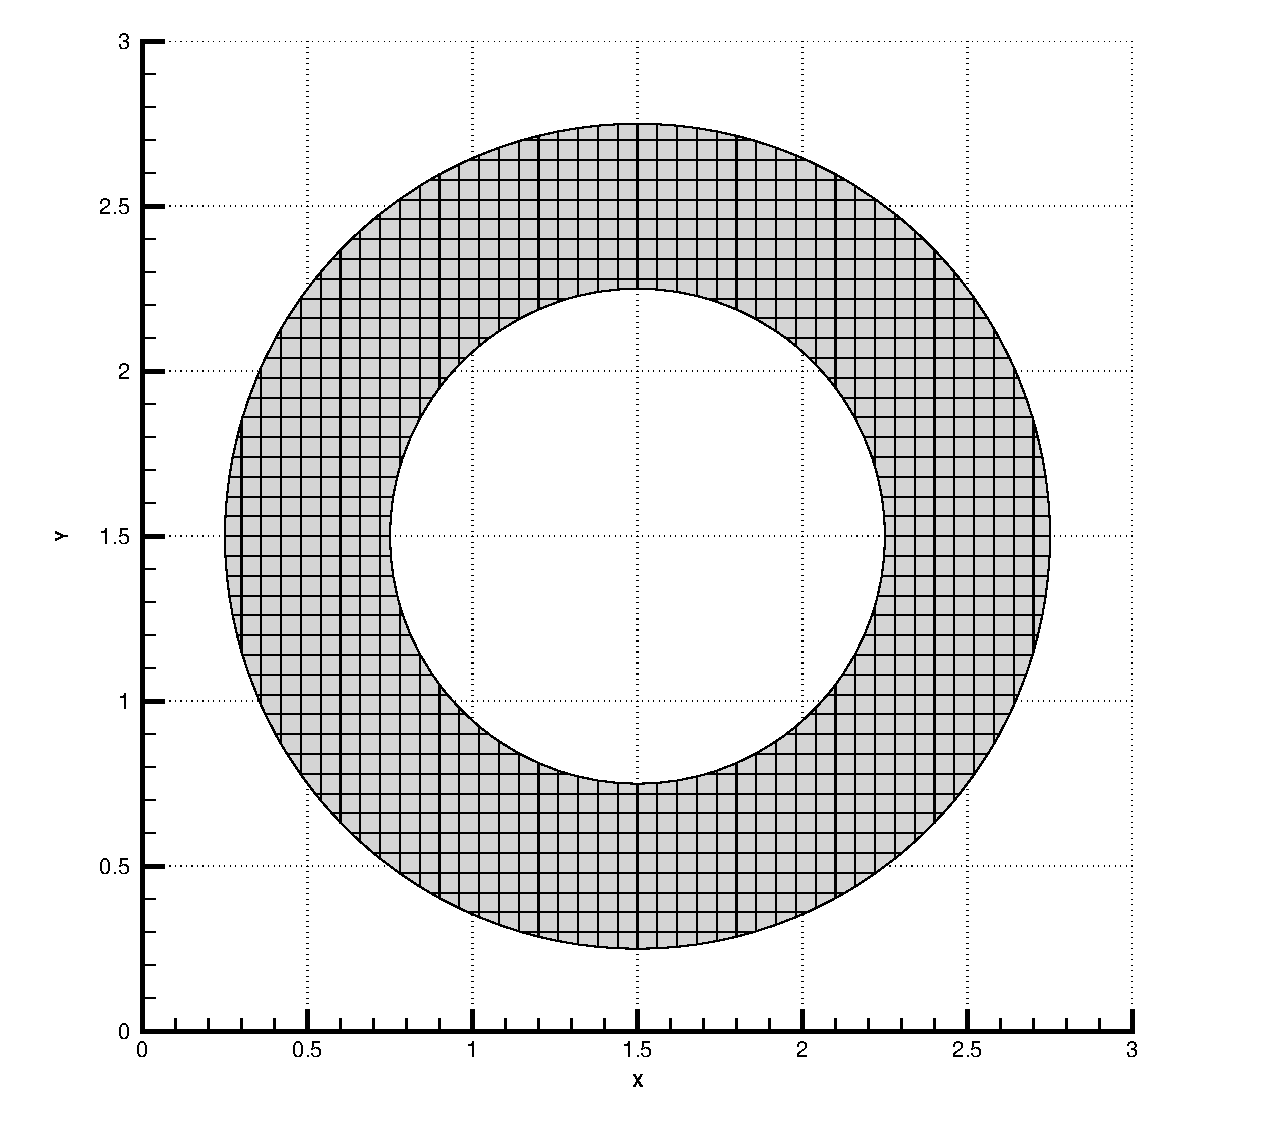
\includegraphics[width = 0.5\linewidth]{figs/rotatinghill_grid.eps} \label{fig:rotatinghillgrid}} 
%	\quad
%	\subfloat[Isolines of exact solution at the initial and final time. SHOW
%	COMPUTED SOLUTION TOO]{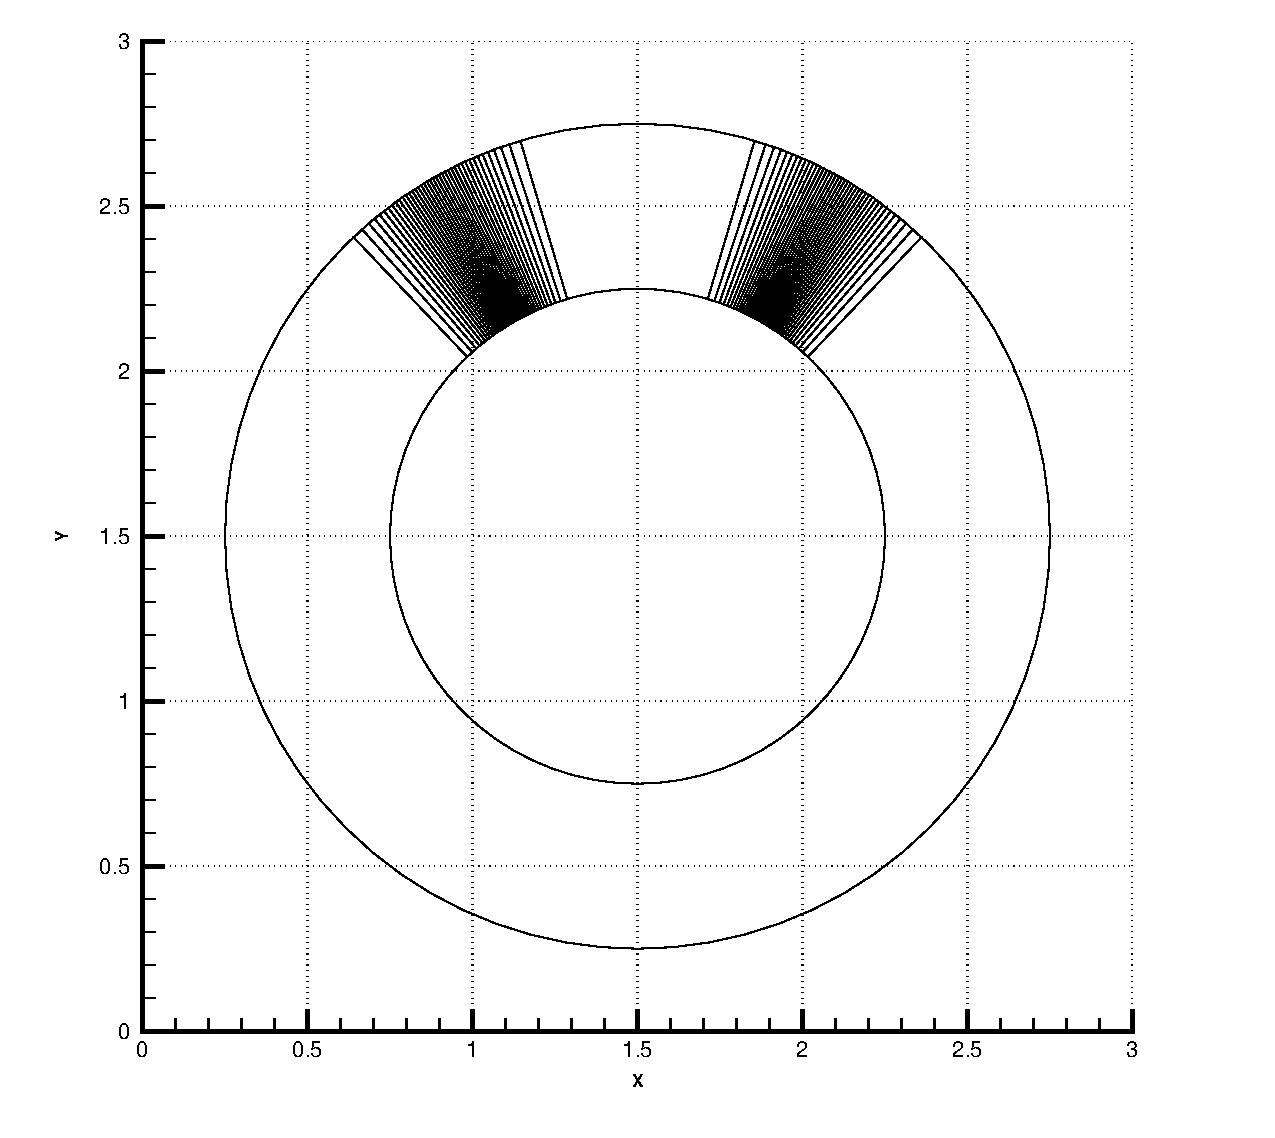
\includegraphics[width = 0.5\linewidth]{figs/rotatinghill_solution.eps}\label{fig:rotatinghillexactiso}}
%\end{figure}
%\begin{figure}
%	\begin{center}
%		%\vspace*{-.5in}
%		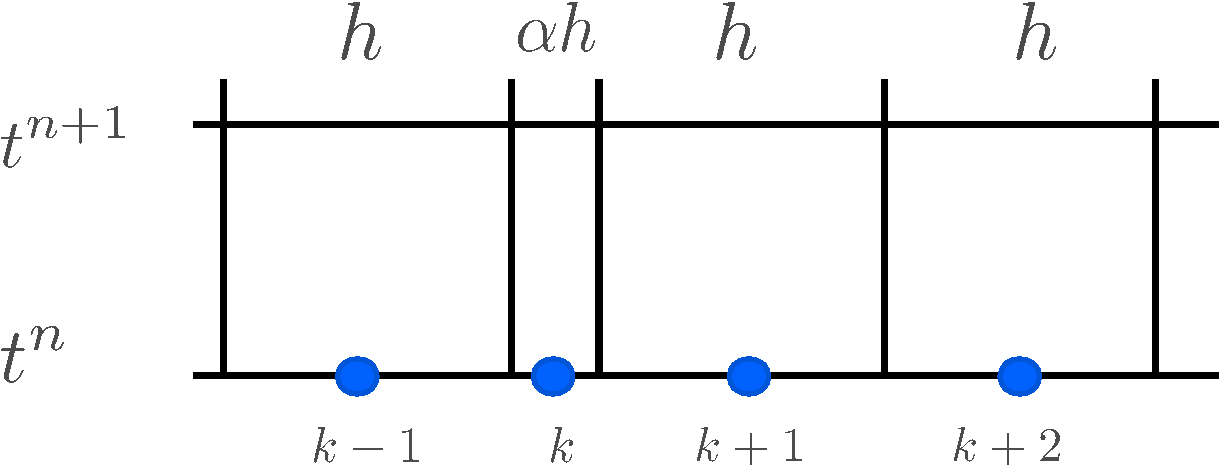
\includegraphics[height=1.3in]{figs/1dfig.pdf}
%		\caption{\sf Notation for model problem in one space dimension. The small
%			cell has size $\alpha h$ in a mesh with regular mesh width $h$.}
%		\label{fig:modelProblem1}
%	\end{center}
%\end{figure}


%To set the stage, notice that cell merging itself can
%be rewritten as a postprocessing step.
%\commentout{
%To take one step to update a finite volume approximation to
%$u_t + u_x = 0$ we do the following:
%\begin{itemize}
%\setlength\itemsep{.2in}
%\item
%{\bf Finite Volume Step}\\
%Take the usual finite volume step with fixed, regular  $\Delta t$ on all cells 
%including the small cell:
%\begin{equation}
%\bar{u}_j = u_j^n - \frac{\Delta t}{h_j} \; (f_{j+1/2} - f_{j-1/2} ), 
%\quad \forall j.
%\label{eqn:fvupdate}
%\end{equation}
%
%\item
%{\bf {\em Temporarily} Create Merged Cell}\\
%Temporarily create the {\em merged} cell $\overline{u_M}$ consisting of the small cell $u_j$ and one
%or both of its neighbors so that it the merged cell is of sufficient
%size (to be discussed later).  For simplicity here we will merge 
%only with the neighbor on the right,
%\begin{equation}
%\widehat{q_M} =  \frac{ h_k \bar{u}_k + h_{k+1} \bar{u}_{k+1} } {h_k +
%h_{k+1}} .
%\label{eqn:mergestep}
%\end{equation}
%
%\item
%{\bf Compute Merge Cell Gradient }\\
%There are several ways to do this. 
%Two simple possibilities are 
%\begin{equation}
%\nabla \widehat{u_M} = \frac{\bar{u}_{k+2} - \bar{u}_{k-1}} {x_{k+2}-x_{k-1}}
%\label{eqn:gradLim1}
%\end{equation}
%which does not use the merged cell,
%or
%\begin{equation}
%\nabla \widehat{u_M} = \frac{\bar{q}_{k+2} - \widehat{u_{M}}} {x_{k+2}-x_{M}}
%\label{eqn:gradLim2}
%\end{equation}
%which uses the merged cell, and $x_M$ is the centroid of the merged
%cell.
%The choice of gradient stencil will be studied later in section \ref{sec:srdAlg}.
%
%%Other more accurate alternatives exist, not all of which are stable.
%%It would be better to use smaller stencils, perhaps including $u_{k+1}$
%%or $\overline{u_M}$ itself.
%
%\item
%{\bf Redistribute Merged State to Cells Comprising Merged cell }\\
%Replace the provisional values computed in the cells comprising the
%merged cell with the merged solution reconstructed to the cell
%centroids:
%\begin{equation}
%\begin{split}
%u_k^{n+1} &= \widehat{u_M} +  (x_k - x_M) \nabla \widehat{u_M}\\
%u_{k+1}^{n+1} &= \widehat{u_M} +  (x_{k+1} - x_M) \nabla \widehat{u_M}
%\end{split}
%\end{equation}
%\end{itemize}
%}
%First update cells $k$ and $k+1$, shown in Figure \ref{fig:modelProblem1},  using a 
%standard finite volume scheme on all cells:
%\begin{equation}
%\bar{u}_j = u_j^n - \frac{\Delta t}{h_j} \; (f_{j+1/2} - f_{j-1/2} ), 
%\quad \forall j.
%\label{eqn:fvupdate}
%\end{equation}
%Next form the merged cell
%\begin{equation}
%\widehat{q_M} =  \frac{ h_k \bar{u}_k + h_{k+1} \bar{u}_{k+1} } {h_k +
%h_{k+1}} .
%\label{eqn:mergestep}
%\end{equation}
%which works out to
%\begin{equation}
%\widehat{q_M} = \widehat{q_M}^n - 
%\frac{\Delta t}{h_k + h_{k+1}} (f_{k+3/2} - f_{k-1/2})
%\end{equation}
%For the simplest first order version, we simply set
%\begin{equation}
%u_k^{n+1} = u_{k+1}^{n+1} = \widehat{q_M} 
%\label{eqn:finalstep}
%\end{equation}
%Recognizing that $h_k+h_{k+1}$ is the merged cell volume makes 
%clear the relationship to cell merging.
%The final update step \eqref{eqn:finalstep} is replaced by 
%\begin{equation}
%\begin{split}
%u_k^{n+1} &= \widehat{q_M} +  (x_k - \widehat{x}_M) \,\,  \widehat{\sigma_M}\\
%u_{k+1}^{n+1} &= \widehat{q_M} +  (x_{k+1} - \widehat{x}_M) \,  \widehat{\sigma_M}
%\end{split}
%\end{equation}
%where $\widehat{\sigma_M}$ is a reconstructed slope on the merged cell.
%The state redistribution method is linearity preserving when the base finite volume scheme and the reconstructed slope on merged cells $\widehat{\sigma_M}$ are accurate enough.
%By using a polynomial of degree $d>1$ and
%including more neighbors in the
%redistribution (on top of a more accurate finite volume scheme for the
%entire mesh),
%we have a path to higher order accuracy.
%The method is also conservative since the mass of the merged cell equals the 
%mass of the two cells comprising it.



%The choice of merging neighborhoods and gradients is what makes up the
%specifics of SRD in two space dimensions. Furthermore, it can happen
%that a cell has more than one neighborhood with
%which it should merge. This is what often causes complications in cell
%merging algorithms. In SRD, we will simply use all such values appropriately
%weighted.
%
%In the next section  we first discuss the finite volume schemes to which SRD will
%be applied.
%The SRD algorithm in two space dimensions will be presented in section
%\ref{sec:srdAlg}.
%For simplicity we present the second order accurate version first.
%The more general higher order extension is described in 
%section \ref{sec:ho}.
%Some theoretical results using one-dimensional model problems are in
%section \ref{sec:theory}. 
%Section \ref{sec:compResults} shows computational results for both smooth
%problems and shocked flow for both linear advection and the Euler equations.  We conclude in section \ref{sec:conc}.
